\chapter{Diseño del Control} \label{chap:Control}
\chapterimage{figuras/ImagenesPortada/PortadaControl.jpg}
\hrule
\vspace{3mm}

El manejo del brazo de una forma adecuada requiere la aplicación de diferentes lazos de control; en este capítulo se detalla el trabajo realizado en esta línea.
\\

El control más básico a realizar sobre un brazo robótico es el control en posición articular: el objetivo es poder introducir una consigna en grados (posición que se quiere alcanzar) que deberá ser alcanzada por el sistema, por cada articulación. El enfoque a seguir para conseguir este tipo de control puede variar en función de los diferentes componentes utilizados; en este caso el diseño de este control se ve fuertemente marcado por los actuadores elegidos, los servos Cytron G15 Cube (vistos en \ref{sec:Electronica:Actuadores}).
\\

Poder controlar la posición de las articulaciones lleva implícito el control del movimiento de las mismas. Esto implica controlar la velocidad a la que se mueven, de forma que, ajustándola se podrá acelerar y desacelerar el movimiento articular para alcanzar, de forma suave las diferentes posiciones articulares deseadas. De esta manera se enlaza un control en posición con un control de velocidad en cascada. La figura \ref{fig:Control:control_cascada} representa el lazo de control completo de posición con un lazo de velocidad integrado. En los siguientes apartados se detalla en concreto cada uno de los lazos representados.


\begin{figure}[H]
    \centering
    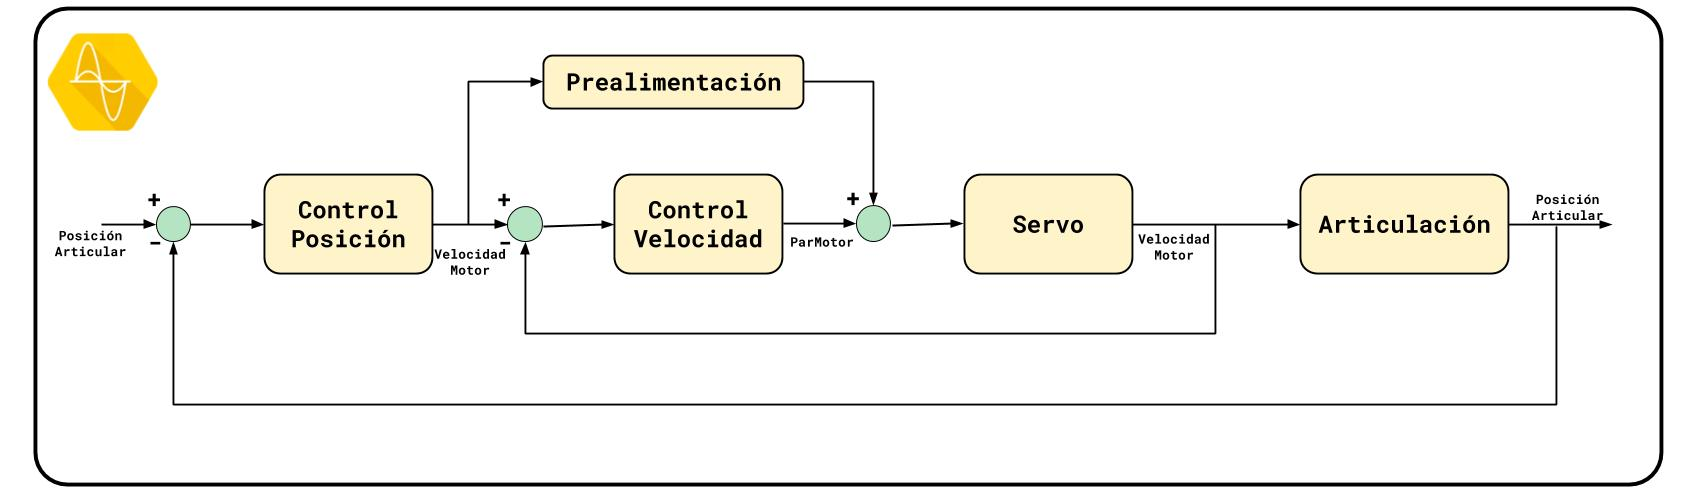
\includegraphics[width=1\textwidth]{figuras/Imagenes_Control/control_cascada.jpg}
    \caption{Control en cascada de Posición + Velocidad}
    \label{fig:Control:control_cascada}
    \immagesource{Autor}
\end{figure}

Este esquema de control se aplica principalmente a las articulaciones dos y tres, que son las que incluyen realimentación de posición. La primera articulación se controlará en posiciones incrementales ajustando a lo comandado por parte de la tablet en el extremo.

\section{Control de velocidad para los servos} \label{sec:Control:velocidad_g15}

La relación entre la velocidad articular y la velocidad de los servos no es directa debido a la cadena de transmisión mecánica por la que pasa el movimiento. El objetivo de controlar la velocidad de la articulación es poder acelerar y desacelerar de forma controlada dicha articulación. En este caso bastará con asegurar que, cuando se pida una velocidad superior o inferior la articulación se comporte en consecuencia, sin ser tan relevante la velocidad real de la articulación. El problema, una vez concretado esto, se reduce a controlar la velocidad de los servos.
\\

Los servos elegidos, aunque poseen un control efectivo de velocidad cuando se configuran en modo posicional (se envían posiciones objetivo en grados a alcanzar), carecen del mismo en un modo de rotación continua. La cadena cinemática construida implica que el servo deberá permitir giro multivuelta en los servos. Por lo tanto es obligatorio utilizar el modo de rotación continua, con un control implementado de par a realizar (aceptando valores mapeados de 0 a 1023).
\\

El lazo de control de velocidad implementado recibe una consigna de velocidad objetivo y actúa sobre el par motor que se enviará al servo.
\\

Puesto que se debe lograr una alta velocidad de respuesta este ajuste no se puede realizar por compensación del error (mediante una acción integral).Como se ha visto en la imagen \ref{fig:Control:control_cascada} la estrategia seguida ha sido la de prealimentar el controlador de velocidad. Esto significa que para cada consigna de velocidad se estimará el par requerido en cadena abierta para luego corregir el posible error y ruido con un controlador tradicional; es decir, se implementará un cálculo de la prealimentación adaptativa que se ajustará según la situación del brazo.
\\

Ajustar dicha prealimentación requiere conocer el comportamiento del servo. En la figura \ref{fig:Control:control_velocidad_par_1}\footnote{Esta gráfica surge de realizar un test de aceleración controlada almacenando los valores de tiempo, par y velocidad. Los valores se recogen de forma discreta a una frecuencia de 100 Hz. Para obtener una gráfica más significativa el test se ha realizado hasta veinte veces para, haciendo la media, obtener una relación estimada de como se comporta el servo de forma \textit{continua}.} se pude ver como se comporta la variación de velocidad del servo en vacío frente a una variación del par requerido. Se pueden reconocer dos etapas en la evolución de dichas variables. En los instantes iniciales la velocidad se mantiene a cero hasta que el par aplicado es capaz de superar el par necesario para mover el servo (superar el rozamiento estático). A partir de ese punto la variación de la velocidad frente al par aplicado si se comporta de manera lineal.

\begin{figure}
    \centering
    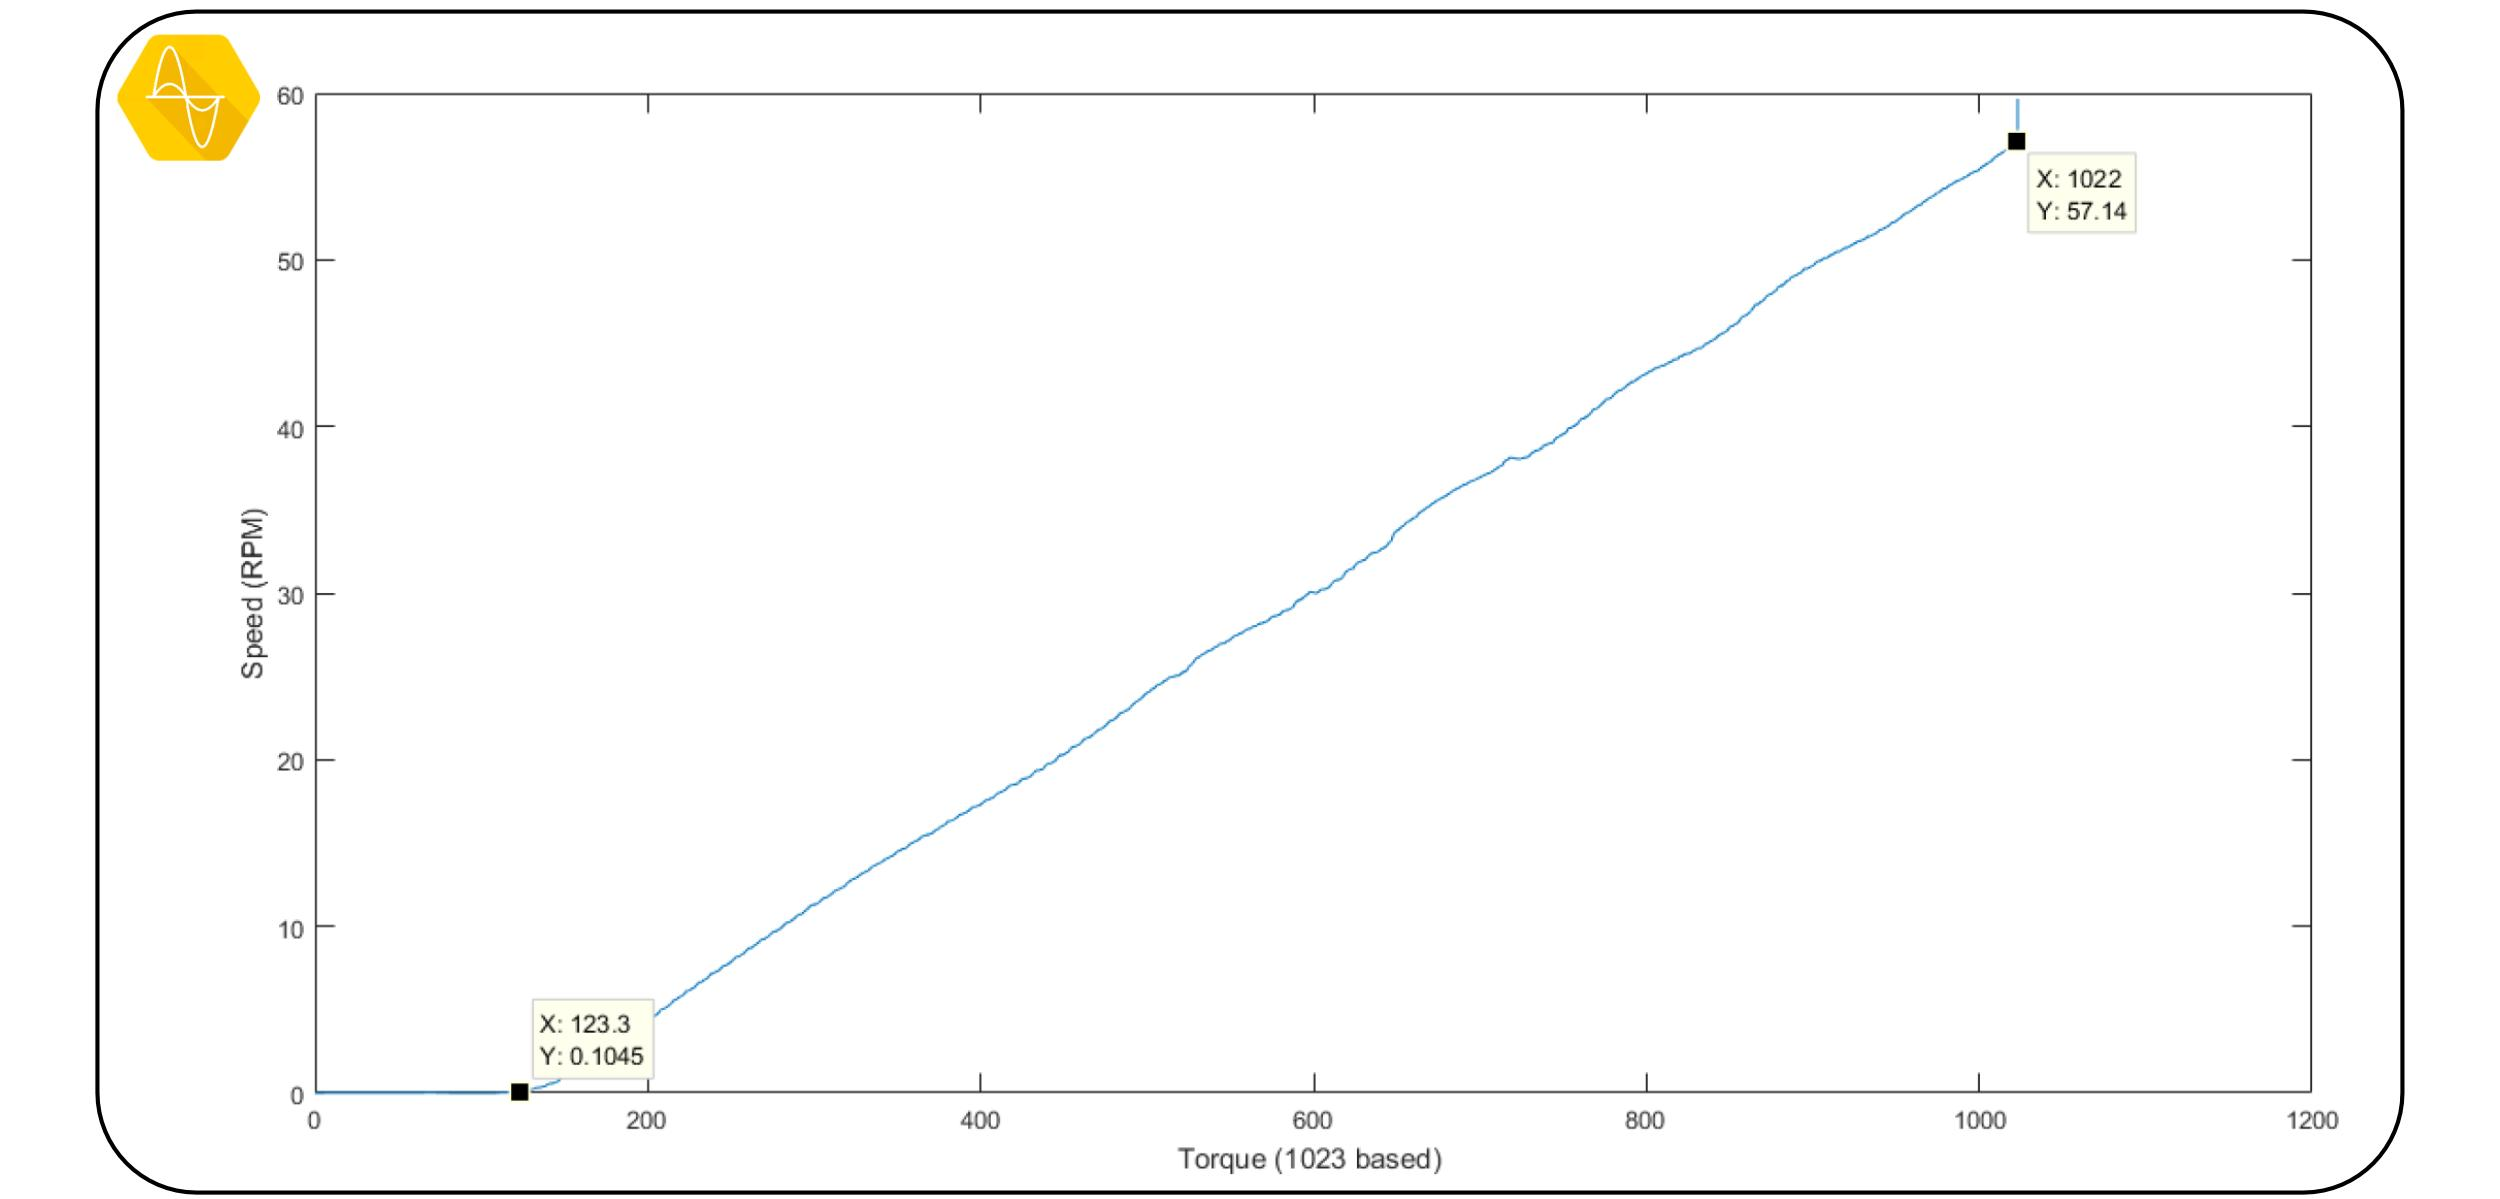
\includegraphics[width=1\textwidth]{figuras/Imagenes_Control/Control_1.jpg}
    \caption{Variación de la velocidad del servo ante variaciones del par aplicado por el mismo}
    \label{fig:Control:control_velocidad_par_1}
    \immagesource{Autor}
\end{figure}

Este comportamiento se repite de forma análoga aplicando diferentes cargas sobre el servo, tal y como puede verse en la figura \ref{fig:Control:control_velocidad_par_2}\footnote{Test de aceleración controlada discretizando los valores a una frecuencia de 100 Hz. El test para cada valor de carga se ha realizado hasta veinte veces obteniéndose una estimación del comportamiento continuo del servo haciendo la media. La carga se ha aplicado en el eje vertical de forma que se mantenga continua a lo largo del test con un montaje del servo similar al que llevará en el brazo robótico.}. Para las diferentes cargas se puede observar una zona en la que, variando el par, la velocidad permanece inalterable (zona en la cual el par aplicado por la carga es superior al aplicado por el servo) y una zona lineal\footnote{Ocurre que el servo, al funcionar en modo multivuelta va almacenando cuerda sobre la polea variando la distancia al eje desde la que se efectúa el par. A cargas elevadas supone una distorsión en el comportamiento esperado. Las repeticiones de los test se han realizado en las mismas condiciones de partida por lo que dichas distorsiones se han mantenido equivalentes en todas ellas}. En la zona de comportamiento lineal, en base a la gráfica mostrada, se puede asumir que la pendiente es igual en todos los casos. Esta deducción concuerda con el hecho de que una vez salvado el peso de la carga, un aumento en el par si debería, físicamente, suponer un aumento proporcional en la velocidad.
\\

\begin{figure}
    \centering
    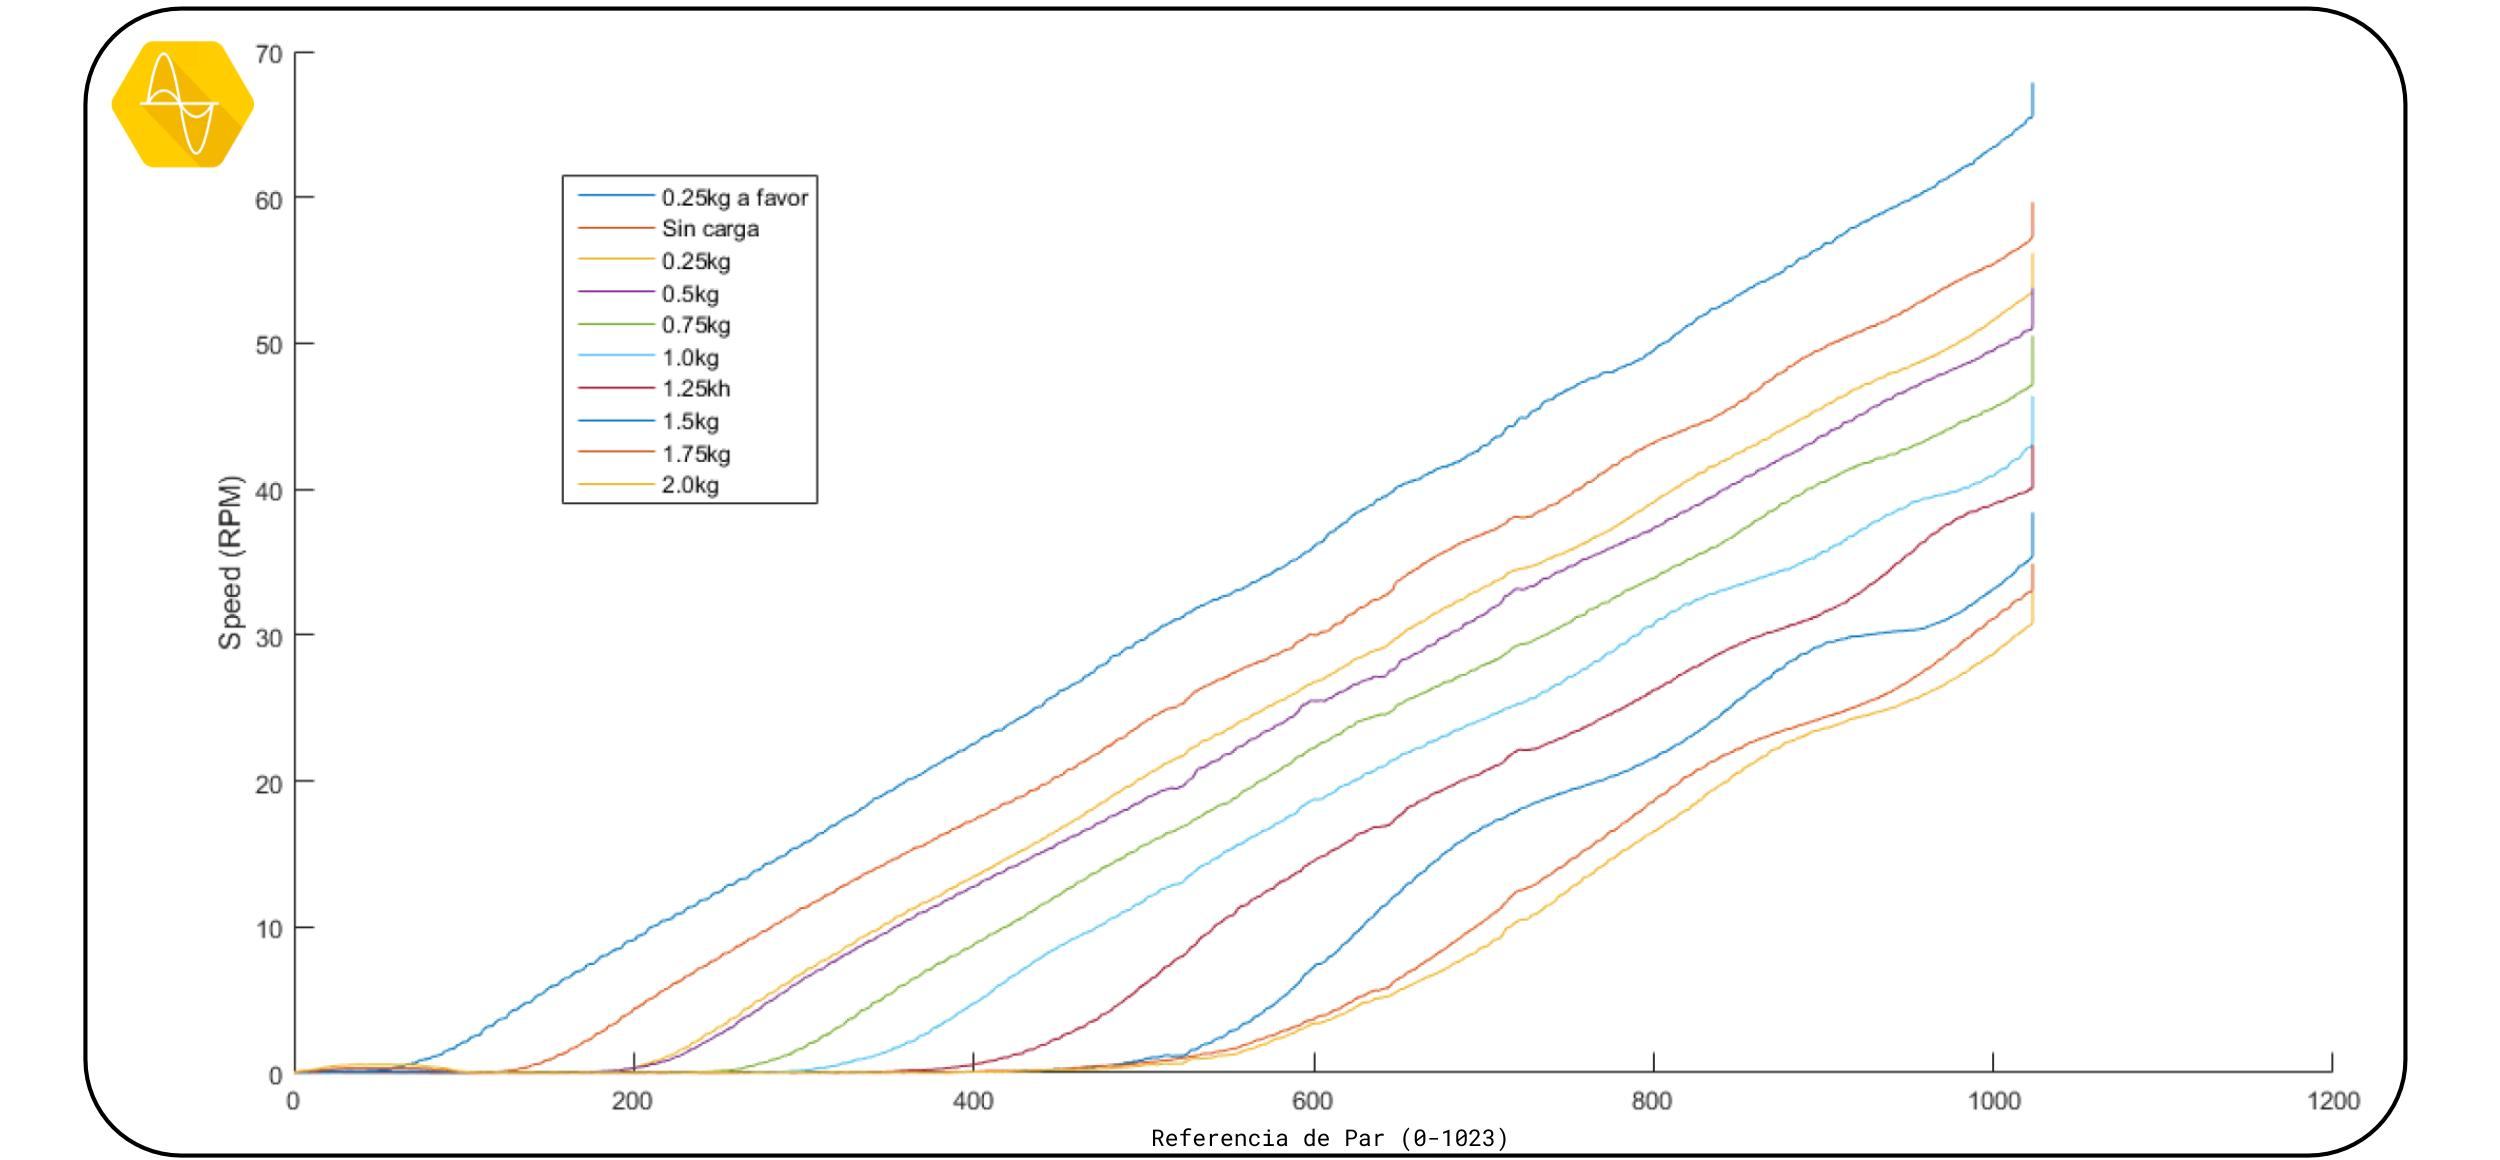
\includegraphics[width=1\textwidth]{figuras/Imagenes_Control/Control_2.jpg}
    \caption{Variación de la velocidad del servo ante variaciones del peso aplicado sobre el mismo}
    \label{fig:Control:control_velocidad_par_2}
    \immagesource{Autor}
\end{figure}

Matemáticamente significa que, conociendo el punto de funcionamiento [par,velocidad] en el que se está trabajando se pude obtener el par necesario para compensar los efectos de la gravedad sobre la el par en el motor. Los servos utilizados permiten leer, entre otros datos, estos dos valores necesarios de forma que en todo momento podemos observar la posición de la situación actual en el plano representado de par frente a velocidad.
\\

Basándose en la representación de la figura \ref{fig:Control:calculo_control} se puede ver, gráficamente como se calcula la prealimentación para el punto (n+1) conocido el punto en el instante (n). Conociendo dicho punto y la pendiente que relaciona la variación de ambos parámetros una vez vencida la gravedad se obtiene el par necesario para vencer dicho par:

\begin{equation}
    Torque_{Compensacion} =  Torque_n - \frac{Velocidad_{n}}{pendiente}
\end{equation}

Conocido dicho valor se puede calcular, desplazándose de vuelta hacia arriba por la recta el valor de par que proporcione la velocidad requerida:

\begin{equation}
    Torque_{n+1} = Torque_{Compensacion} - \frac{Velocidad_{target}}{pendiente}
\end{equation}

\begin{figure}[H]
    \centering
    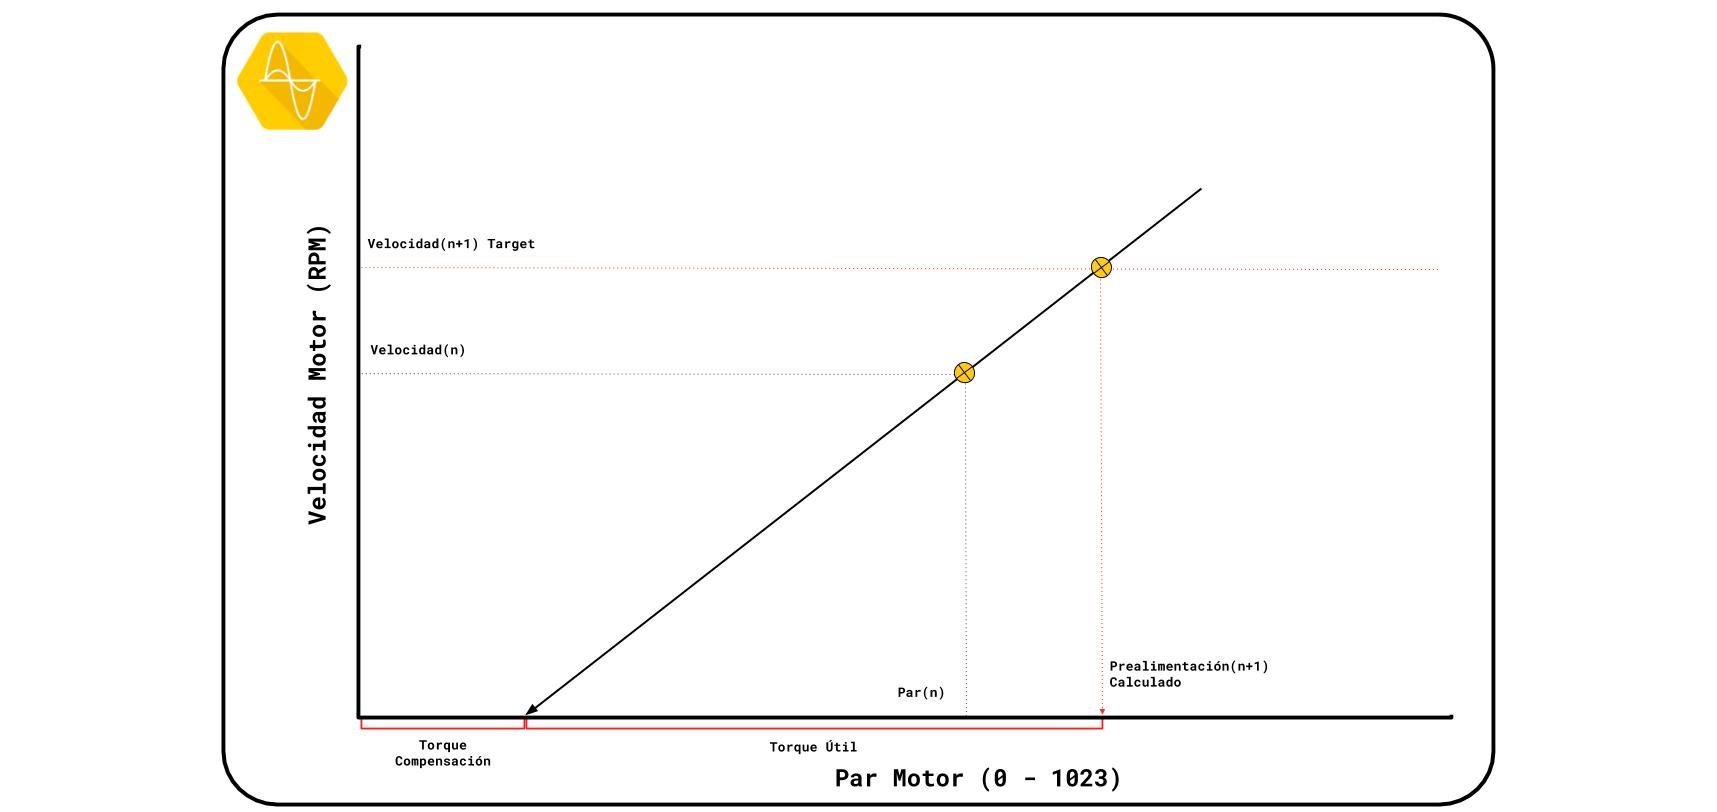
\includegraphics[width=1\textwidth]{figuras/Imagenes_Control/calculo_control.jpg}
    \caption{Cálculo matemático de la prealimentación adaptativa.}
    \label{fig:Control:calculo_control}
    \immagesource{Autor}
\end{figure}

Este método de calcular la prealimentación a través de un observador del estado del servo conlleva cierto error en la medida obtenida en base a que la información se obtiene de forma discreta de igual forma que la actualización del par. La frecuencia a la que se actualizan dichos valores es lo suficientemente rápida como para que el efecto sea mínimo. Aún así, posible error así como ruidos o perturbaciones externas son absorbidas por la segunda parte del control en velocidad descrito: el regulador PID implementado.
\\

A continuación se añade un regulador que podrá absorber ruido y ayudar a reaccionar ante perturbaciones externas. El regulador implementado es un regulador PID estándar cuyas constantes (constante proporcional, integral y derivativa) se han ajustado de forma experimental. Debido a la prealimentación el regulador queda reducido a una acción de tipo PD, con unas constantes kp = 3 y kd = 1.
\\

La frecuencia a la que funciona el lazo de control de velocidad está limitada por el tiempo que se tarda en comunicar toda la información entre el sistema y los servos.
\\

Los servos aceptan valores de par hasta 1023. Se ha limitado el regulador  de forma que satura en dicho valor manteniendo el valor máximo de manera constante hasta que el valor sea inferior al mencionado.

\section{Control de posición articular} \label{sec:Contorl:posicion_articular}

El control de posición articular recibe una consigna de posición a alcanzar y la \textit{transforma} en una consigna de velocidad para el servo. Para que el control en cascada funcione correctamente el lazo de control de velocidad ha de ser más rápido que el de posición, concretamente el lazo de control de posición funciona a una frecuencia 10 veces inferior al lazo de control de velocidad.
\\

El regulador PID implementado se encarga de llevar la articulación al punto deseado. Es importante asegurar que conforme se acerca al punto de consigna se desacelere de forma que se eviten oscilaciones provocadas por los muelles que compensan la carga de la segunda y tercera articulación.
\\

Aunque los servos pueden alcanzar una velocidad de 65 revoluciones por minuto en vacío se ha establecido un máximo de 30 rpm a la salida de este regulador. De esta forma la velocidad del brazo depende de la salida del regulador impidiendo así que se vea afectada por la posición o carga del mismo.
\\

El regulador, que tras el ajuste experimental ha resultado ser un PD tiene por constantes los siguientes valores: kp = 5; kd = 0.2.
